%%
%% This is file `sample-acmlarge.tex',
%% generated with the docstrip utility.
%%
%% The original source files were:
%%
%% samples.dtx  (with options: `all,journal,bibtex,acmlarge')
%% 
%% IMPORTANT NOTICE:
%% 
%% For the copyright see the source file.
%% 
%% Any modified versions of this file must be renamed
%% with new filenames distinct from sample-acmlarge.tex.
%% 
%% For distribution of the original source see the terms
%% for copying and modification in the file samples.dtx.
%% 
%% This generated file may be distributed as long as the
%% original source files, as listed above, are part of the
%% same distribution. (The sources need not necessarily be
%% in the same archive or directory.)
%%
%%
%% Commands for TeXCount
%TC:macro \cite [option:text,text]
%TC:macro \citep [option:text,text]
%TC:macro \citet [option:text,text]
%TC:envir table 0 1
%TC:envir table* 0 1
%TC:envir tabular [ignore] word
%TC:envir displaymath 0 word
%TC:envir math 0 word
%TC:envir comment 0 0
%%
%% The first command in your LaTeX source must be the \documentclass
%% command.
%%
%% For submission and review of your manuscript please change the
%% command to \documentclass[manuscript, screen, review]{acmart}.
%%
%% When submitting camera ready or to TAPS, please change the command
%% to \documentclass[sigconf]{acmart} or whichever template is required
%% for your publication.
%%
%%

\documentclass[acmlarge]{acmart}
%%
%% \BibTeX command to typeset BibTeX logo in the docs
\AtBeginDocument{%
  \providecommand\BibTeX{{%
    Bib\TeX}}}

%% Rights management information.  This information is sent to you
%% when you complete the rights form.  These commands have SAMPLE
%% values in them; it is your responsibility as an author to replace
%% the commands and values with those provided to you when you
%% complete the rights form.
\setcopyright{acmlicensed}
\copyrightyear{2018}
\acmYear{2018}
\acmDOI{XXXXXXX.XXXXXXX}

%%
%% These commands are for a JOURNAL article.
\acmJournal{POMACS}
\acmVolume{37}
\acmNumber{4}
\acmArticle{111}
\acmMonth{8}

%%
%% Submission ID.
%% Use this when submitting an article to a sponsored event. You'll
%% receive a unique submission ID from the organizers
%% of the event, and this ID should be used as the parameter to this command.
%%\acmSubmissionID{123-A56-BU3}

%%
%% For managing citations, it is recommended to use bibliography
%% files in BibTeX format.
%%
%% You can then either use BibTeX with the ACM-Reference-Format style,
%% or BibLaTeX with the acmnumeric or acmauthoryear sytles, that include
%% support for advanced citation of software artefact from the
%% biblatex-software package, also separately available on CTAN.
%%
%% Look at the sample-*-biblatex.tex files for templates showcasing
%% the biblatex styles.
%%

%%
%% The majority of ACM publications use numbered citations and
%% references.  The command \citestyle{authoryear} switches to the
%% "author year" style.
%%
%% If you are preparing content for an event
%% sponsored by ACM SIGGRAPH, you must use the "author year" style of
%% citations and references.
%% Uncommenting
%% the next command will enable that style.
%%\citestyle{acmauthoryear}


%%
%% end of the preamble, start of the body of the document source.
\usepackage{graphicx}
\usepackage{subcaption}
\graphicspath{{Figures/}}
\begin{document}

%%
%% The "title" command has an optional parameter,
%% allowing the author to define a "short title" to be used in page headers.
% 
\title{Medication Adherence Challenges and Design Directions for Older Adults and Caregivers in Bangladesh: From Formative Study to Prototype Evaluation}

%%
%% The "author" command and its associated commands are used to define
%% the authors and their affiliations.
%% Of note is the shared affiliation of the first two authors, and the
%% "authornote" and "authornotemark" commands
%% used to denote shared contribution to the research.

\author{Bir Ballav Roy}
\authornotemark[1]
\affiliation{%
  \institution{BRAC University}
  \city{Dhaka}
  \state{Dhaka}
  \country{Bangladesh}
}

% \author{Lars Th{\o}rv{\"a}ld}
% \affiliation{%
%   \institution{The Th{\o}rv{\"a}ld Group}
%   \city{Hekla}
%   \country{Iceland}}
% \email{larst@affiliation.org}

% \author{Valerie B\'eranger}
% \affiliation{%
%   \institution{Inria Paris-Rocquencourt}
%   \city{Rocquencourt}
%   \country{France}
% }

% \author{Aparna Patel}
% \affiliation{%
%  \institution{Rajiv Gandhi University}
%  \city{Doimukh}
%  \state{Arunachal Pradesh}
%  \country{India}}

% \author{Huifen Chan}
% \affiliation{%
%   \institution{Tsinghua University}
%   \city{Haidian Qu}
%   \state{Beijing Shi}
%   \country{China}}

% \author{Charles Palmer}
% \affiliation{%
%   \institution{Palmer Research Laboratories}
%   \city{San Antonio}
%   \state{Texas}
%   \country{USA}}
% \email{cpalmer@prl.com}

% \author{John Smith}
% \affiliation{%
%   \institution{The Th{\o}rv{\"a}ld Group}
%   \city{Hekla}
%   \country{Iceland}}
% \email{jsmith@affiliation.org}

\author{Jannatun Noor Mukta}
\affiliation{%
  \institution{BRAC University}
  \city{Dhaka}
  \country{Bangladesh}}
\email{jpkumquat@consortium.net}

%%
%% By default, the full list of authors will be used in the page
%% headers. Often, this list is too long, and will overlap
%% other information printed in the page headers. This command allows
%% the author to define a more concise list
%% of authors' names for this purpose.
\renewcommand{\shortauthors}{Trovato et al.}

%%
%% The abstract is a short summary of the work to be presented in the
%% article.

\begin{abstract}
\section*{Abstract}
  Older adults juggle complicated medication schedules, often relying on memory, habit, and the quiet labor of family. Routines can break due to some external scenarios rather than internal qualities. An abundance of tools exist to promise help with adherence, yet their shortcomings fail for widespread and long-term adoption. We interviewed 26 participants, 17 older adults and 9 caregivers in Bangladesh to understand how their medications are really managed, their access and experience with contemporary technology, and how people imagine voice reminder based solutions might help. A clear enthusiasm was shown for relevant technological solutions that may add to routines, not override. What we found reframes the problem: memory is a matter of dignity as much as risk, adherence is fragile, and on top of autonomy, caregiving is often aided by family members. We discuss possible implications and directions regarding building on top of these findings towards a useful solution.
\end{abstract}

%%
%% The code below is generated by the tool at http://dl.acm.org/ccs.cfm.
%% Please copy and paste the code instead of the example below.
%%
\begin{CCSXML}
<ccs2012>
   <concept>
       <concept_id>10003120.10003121.10003122.10003334</concept_id>
       <concept_desc>Human-centered computing~User studies</concept_desc>
       <concept_significance>500</concept_significance>
       </concept>
 </ccs2012>
\end{CCSXML}

\ccsdesc[500]{Human-centered computing~User studies}
% \begin{CCSXML}
% <ccs2012>
%  <concept>
%   <concept_id>00000000.0000000.0000000</concept_id>
%   <concept_desc>Do Not Use This Code, Generate the Correct Terms for Your Paper</concept_desc>
%   <concept_significance>500</concept_significance>
%  </concept>
%  <concept>
%   <concept_id>00000000.00000000.00000000</concept_id>
%   <concept_desc>Do Not Use This Code, Generate the Correct Terms for Your Paper</concept_desc>
%   <concept_significance>300</concept_significance>
%  </concept>
%  <concept>
%   <concept_id>00000000.00000000.00000000</concept_id>
%   <concept_desc>Do Not Use This Code, Generate the Correct Terms for Your Paper</concept_desc>
%   <concept_significance>100</concept_significance>
%  </concept>
%  <concept>
%   <concept_id>00000000.00000000.00000000</concept_id>
%   <concept_desc>Do Not Use This Code, Generate the Correct Terms for Your Paper</concept_desc>
%   <concept_significance>100</concept_significance>
%  </concept>
% </ccs2012>
% \end{CCSXML}

% \ccsdesc[500]{Do Not Use This Code~Generate the Correct Terms for Your Paper}
% \ccsdesc[300]{Do Not Use This Code~Generate the Correct Terms for Your Paper}
% \ccsdesc{Do Not Use This Code~Generate the Correct Terms for Your Paper}
% \ccsdesc[100]{Do Not Use This Code~Generate the Correct Terms for Your Paper}

% %%
% %% Keywords. The author(s) should pick words that accurately describe
% %% the work being presented. Separate the keywords with commas.
% \keywords{Do, Not, Use, This, Code, Put, the, Correct, Terms, for,
%   Your, Paper}

\received{20 February 2007}
\received[revised]{12 March 2009}
\received[accepted]{5 June 2009}

%%
%% This command processes the author and affiliation and title
%% information and builds the first part of the formatted document.
\maketitle

\newpage
\section{Introduction}
Older adults are living with multiple chronic health problems, which means they often have to maintain complex medication schedules. Forgetting a pill or taking it at the wrong time is a common risk, which is made worse by age-related changes to memory,
eyesight, and physical ability. These mistakes are harmful: they lead to worse health, more
hospital visits, and higher medical costs. This makes helping older adults take their medicine
correctly a major public health goal.
We already know that social factors play a big role in these routines \cite{Bastani01122021}. We also know that
older adults often struggle to use new health technologies \cite{Ahmad2022}, and that their willingness to try
depends on whether they see a tool as useful, easy, and socially acceptable \cite{info:doi/10.2196/65269}. A person's
own background and abilities also affect whether they stick with a technology long-term \cite{10.1093/geront/gny113}.
But even when a technology seems promising, basic design flaws often stop it from working
well in the real world \cite{10.1145/174800.174808}. The takeaway is simple: people not taking their medicine correctly
is both a medical problem and a design problem. We need solutions that fit into the actual
lives, abilities, and support networks of older people and their caregivers \cite{info:doi/10.2196/65776}, \cite{TURJAMAA2020677}, \cite{10.1007/978-3-642-02774-1_77}.
Today, there are many digital tools like smartphone apps and smart pillboxes designed to
help. The problem is, most of them don’t work well for older adults. Many popular apps are
hard to navigate or have text that’s too small, causing users to lose trust and give up \cite{doi:10.1177/1541931213601769}, \cite{10.1145/2556288.2557079}.
Another issue is how they give reminders. Most apps use alarms set for a specific time, but
people often take their medicine with meals or as part of a routine, like “after breakfast” \cite{10.1145/3636534.3698116}.
Voice assistants and AI tools seem like a good alternative, but they come with their own
problems like privacy risks, unreliability, and a lack of personalization \cite{10.1145/3623809.3623827}, \cite{10.1145/3706598.3713578}. Recent
studies show that older adults will only adopt these AI systems if they’ve used similar tech
before and feel the new tool respects their independence and fits their lifestyle \cite{10.1145/3700794.3700803}, \cite{10.1007/978-3-031-24667-8_7}.

All of this points to three big, unsolved problems:

\begin{enumerate}
\def\labelenumi{\arabic{enumi}.}
\item
  Most technology ignores people who have low literacy or use basic
  button phones, not smartphones.
\item
  Caregivers are rarely included in the design process.
\item
  We lack simple, flexible tools that combine voice, visual cues, and
  offline support to match how people actually live.
\end{enumerate}

So, we set out to answer four questions:

\begin{enumerate}
\def\labelenumi{\arabic{enumi}.}
\item
  How do older adults and their caregivers currently manage medications,
  and what are their biggest challenges?
\item
  How do literacy, phone type, and access to technology shape how people
  use these tools?
\item
  What do older adults and caregivers really think, want, and worry
  about when it comes to AI voice reminders?
\item
  How can we design a better system using voice and visuals that works
  for low-literacy and low-tech users? How to retain the users for
  long-term support and adoption?
\end{enumerate}

To answer these questions, we talked to 24 people in semi-structured
interviews. This group included older adults and the family members or
professional caregivers who help them. Our goal was not to test a
specific gadget. We wanted to understand how people manage medications
in their daily lives, how things like literacy and the phones they use
affect them, and what they really think about using AI voice alerts for
reminders. We analyzed our interview notes to find common themes, an
approach grounded in prior HCI work that values understanding real-world
context \cite{Ahmad2022}, \cite{info:doi/10.2196/65269}, \cite{Bastani01122021}. From these themes, we developed a set of
practical design requirements.

This work makes three main contributions. First, we provide a real-world
look at how medication schedules are managed day-to-day. Second, we show
how literacy, device access, and caregiver involvement affect whether
technology helps or hurts. Third, we translate what users told us about
their hopes and fears for AI voice reminders into clear design
principles. In the end, our research aims to close the gap between what
new technology can do and what people actually find useful. We offer a
blueprint for a voice-first system that respects user routines, includes
caregivers, and works for everyone---even those with low literacy or
without a reliable internet connection \cite{10.1145/3623809.3623827}, \cite{10.1145/3706598.3713578}, \cite{10.1145/3700794.3700803}.

\section{Related Work}
Designing technology for older adults has never been only about building
new tools. It is about understanding everyday routines, anxieties, and
motivations, then shaping systems that fit into that reality. Research
spans a wide spectrum---from explaining why adoption fails to
experimenting with AI-driven companions---but the lesson is steady: the
best technology is created with older adults, not for them.

\subsection{Adoption and Everyday Practice}
Older adults face barriers that go well beyond usability. Distrust in
new systems, fears over privacy, low digital confidence, and uneven
access to devices are all common \cite{Ahmad2022}. Whether someone chooses to
adopt often comes down to two judgments: \emph{Is this useful? Is it
simple enough to try?} \cite{info:doi/10.2196/65269}. Social networks also matter. Family and
friends can push adoption as much as interface design \cite{info:doi/10.2196/65269}. At the
same time, older adults are not passive. Many make deliberate choices,
keeping only technologies that fit existing routines and the kind of
support they can realistically expect \cite{10.1093/geront/gny113}, \cite{10.1007/978-3-319-20892-3_47}.

Researchers agree on one point: successful systems require participation
from older adults from the start \cite{10.1007/978-3-540-70540-6_2}, \cite{10.1007/978-3-031-92707-2_9}. Participatory design
shifts them from test subjects to active contributors \cite{10.1145/3357155.3358471}. This may
happen through workshops, co-design sessions, or direct prototype
building \cite{WERNER20223680}, \cite{10.1145/3240925.3240929}. Importantly, people with prior experience using a
system provide more practical and critical feedback than first-time
users \cite{10.1145/3240925.3240929}. Such approaches consistently lead to designs that feel
relevant and usable in real life, not just in lab settings \cite{10.1145/3517428.3544830}, \cite{10.1145/3544548.3580893}.


\subsection{Medication Management}

Medication adherence remains one of the most studied challenges.
Multiple prescriptions and complex schedules are common, and forgetting
doses can cause serious harm \cite{10.1145/3154862.3154883}, \cite{doi:10.1177/2333721419845179}, \cite{10.1145/3636534.3698116}, \cite{Bastani01122021}. Technology has been
tested at several levels.

\emph{Apps and reminders.} Many solutions are smartphone-based \cite{10.1007/978-3-642-02774-1_77},
\cite{10.1145/2556288.2557079}. These range from simple alarms to platforms integrated into apps
like WeChat \cite{10.1145/3630138.3630553}. Problems remain: confusing navigation, small
fonts, or poor accessibility \cite{doi:10.1177/1541931213601769}. More fundamentally, time-based
reminders often misalign with lived routines. Many medications are taken
``with food'' or ``before sleep,'' not strictly at 8 a.m. \cite{10.1145/3636534.3698116}.
Systems that link prompts to daily routines and visualize progress show
stronger results \cite{10.1007/s00779-020-01420-4}, \cite{NIE2024100076}, \cite{10.1145/2556288.2557079}, \cite{10.1145/3462676.3462684}. The best examples are those
co-designed with older adults, producing tools that feel more like
support than constant interruption \cite{10.1145/2491148.2491155}, \cite{FERREIRA2014398}, \cite{Nguyen2023-ku}.

\emph{Devices and sensing.} Not all approaches rely on screens. Smart
pillboxes record openings and share data with caregivers or clinicians
\cite{doi:10.1177/2333721419845179}, \cite{Paul2024-jk}, \cite{TURJAMAA2020677}. Ambient displays, using light or sound, give immediate
feedback without requiring any manual action \cite{info:doi/10.2196/14680}, \cite{10.1145/2556288.2557210}. These
lightweight cues often help build adherence habits \cite{10.1145/2556288.2557210}. More
complex systems use sensors in the home or social platforms for gentle
nudges from relatives \cite{10.1016/j.comcom.2015.04.001}. At the edge of experimentation,
ingestible sensors confirm adherence biologically by transmitting
signals once a pill dissolves \cite{10.1145/2769493.2769570}, \cite{10.1145/3290605.3300806 }. They are effective but raise
obvious questions about privacy and invasiveness.

\subsection{AI, Voice, and Robotics}
AI-driven systems have extended the scope of what support can look like.
The field has moved from static reminders toward personalized,
conversational, and adaptive tools.

\emph{Attitudes toward AI.} Older adults approach AI with cautious
interest. Many see its promise in maintaining independence \cite{10.1145/3706599.3720033}, \cite{10.1145/3565698.3565774},
\cite{info:doi/10.2196/66778}. But concerns are clear: privacy, lack of transparency, and loss
of control \cite{10.1145/3565698.3565774}, \cite{info:doi/10.2196/65776}. Most participants insist AI should assist---not
replace---the role of doctors and caregivers \cite{info:doi/10.2196/66778}.

\emph{Voice interaction.} Voice assistants sidestep screen complexity
and open up interaction through speech \cite{10.1145/3623809.3623827}. They can walk users
through exercises, deliver medication reminders, or read social updates
\cite{info:doi/10.2196/26361}, \cite{10.1145/3623809.3623827}, \cite{10.1145/3517428.3544830}, \cite{10.1007/978-3-031-24667-8_7}. The critical element is personalization. A
well-designed system respects autonomy and adapts to context; a poorly
designed one becomes overbearing and is quickly abandoned \cite{10.1145/3706598.3713839}.
Large language models expand possibilities, making it easier to explain
medical information or allow users to configure their own conversational
agents \cite{10.1145/3706598.3714219}, \cite{10.1145/3706598.3713839}. But reliability remains an issue. Users have
reported repetitive answers, misinformation, and cultural insensitivity
\cite{Enam24032025}, \cite{10.1007/s10514-025-10190-y}, \cite{10.1007/978-3-031-91760-8_6}, \cite{10.1145/3712275}, \cite{10.1145/3700794.3700803}.

\emph{Robotics.} Robots serve dual purposes: practical support and
social companionship. They provide reminders, health monitoring, and
cognitive exercises \cite{10.1145/3533726}, \cite{10.1145/3706599.3719760}. They also offer presence, helping to
reduce loneliness and connect residents with family \cite{10.1145/3638380.3638412}, \cite{10.1145/3610978.3638378}. Design
is decisive here. Robots seen as intrusive or alien fail quickly
\cite{10.1145/3711936}. Robots shaped through participatory processes, with input from
residents and caregivers, achieve higher acceptance and more meaningful
use \cite{10.1145/3533726}, \cite{10.1145/3544548.3580893}.

\textbf{\\
} Taken together, these studies highlight a single pattern. Adoption is
not a matter of building better reminders or adding more features. It
depends on whether the technology fits into everyday routines, respects
autonomy, and is shaped by those who will actually use it. From
pillboxes to voice agents to robots, the most successful work emerges
when researchers design \emph{with} older adults.


\section{Methodology~}
Our study was designed to understand the real-world challenges older
adults and their caregivers face with medication management. We chose a
qualitative approach because we wanted to hear people's stories in their
own words. Instead of starting with a piece of technology, we started
with people's lives, a method that puts human needs first and is known
to be effective when designing for older adults \cite{FERREIRA2014398}, \cite{10.1145/3357155.3358471}, \cite{10.1007/978-3-031-92707-2_9}, \cite{10.1145/3700794.3700803}.
Our main goal was to listen and learn, so we could build a clear picture
of their daily routines, their problems, and what they truly need from a
support tool \cite{10.1145/174800.174808}.

\subsection{Participant Recruitment}
~We talked to a total of 26 participants, 17 of them were older adults, and 9 of them were caregivers. This group was a mix of older adults who manage their own medications and caregivers, primarily family
members, who help them. We specifically looked for people, primarily older adults who are above the age of 40, from different backgrounds to make sure our findings weren't limited to just one group. We sought out individuals with varying levels of comfort with technology, from those who used smartphones daily to those who only used basic phones or no mobile phone at all. We also made an effort to include people with different literacy levels, as this is often a barrier to using health technology \cite{10.1145/3706598.3713617}. We continued recruiting people until we started hearing the same stories and themes over and over, which told us we had a solid understanding of the main issues.~

\subsection{Data Collection: Semi-Structured Interviews~}
Our main way of gathering information was through semi-structured
interviews. This just means we had a list of questions to guide the
conversation, but we let each talk flow naturally \cite{10.1145/3411764.3445702}, \cite{10.1145/3565698.3565774}, \cite{10.1145/3706598.3713839}.
Interviews took between 4 minutes to 10 minutes to complete based on the
questions. This flexible style helped people feel comfortable and share
details they might not have in a strict survey.

We asked questions about four main areas:~

Current Routines: We asked them to walk us through a typical day of
managing medications. What tools do they use now, if they do so? What
works and what doesn't for them while managing medication, the primary
instituition was to infer whether or not tech usage is even relevant for
some.~

Challenges and Workarounds: We asked about mistakes, frustrations, and
the clever tricks they've developed to remember their pills.~

Technology Use: We talked about the phones and other devices they use in
daily life. We wanted to know what they felt comfortable with and what
they avoided \cite{10.1145/3712275}. Perceptions of AI and Voice Assistants: We
described a system that could send voice reminders and asked for their
honest thoughts. What were their hopes? What were their expectations
\cite{10.1145/3623809.3623827}, \cite{10.1145/3706598.3713578}?~

We conducted interviews in the place where each participant felt most
comfortable---usually their home. This allowed us to see their
medication setups firsthand and understand their environment better.
With their permission, we took audio recordings and detailed notes
during each conversation. No video was recorded.

\subsection{Data Analysis: Finding the Key Themes~}
After the interviews, our research team worked together to make sense of
everything we had heard. We used a method called thematic analysis
\cite{info:doi/10.2196/65776}, \cite{10.1145/3546743}. First, we transcribed the audio recordings and reviewed
our notes. Then, each member of our team read through all the
transcripts independently, highlighting quotes and phrases that stood
out. We paid close attention to stories, opinions, and problems that
came up repeatedly. Next, we came together as a group. We compared our
notes and started organizing the highlighted ideas into categories.For example, we grouped together all the comments about concerns, suggestions, and placed the stories of caregivers helping with technology into another. Over time, these smaller clusters grew into broader themes—the core ideas that connected everyone’s experiences \cite{Bastani01122021}. This process of coding and organizing helped us move from 26 individual stories to a clear picture of what users truly need. Throughout the study, we also took care to uphold ethical standards: every participant gave informed consent after we explained the purpose of the research and emphasized that their involvement was completely voluntary.
 They could stop the
interview at any time for any reason. To protect their privacy, we used
pseudonyms in all our notes and reports \cite{Ahmad2022}, \cite{info:doi/10.2196/66778}. Building a trusting
relationship was our top priority, as it was the only way to get honest
insights into their lives and needs.

\section{Findings}
Our interviews with older persons and their caregivers revealed that
medication management is not an isolated task but a collective practice
interwoven with memory, habits, familial connections, and aspirations
for future technology assistance. We identified the overarching theme
that emerged from these accounts, which we organized into four main
categories: (1) Reliance on Memory and Habits, (2) Everyday Challenges
in Medication Adherence, (3) The Role of Family and Care Networks, and
(4) Aspirations for Technology-Supported Solutions. Each topic
highlights how older people are now dealing with the daily stress of
managing their medicines while also thinking about what technology might
be like in the future.

\subsection{Reliance on Memory and Habits}
One participant expressed strong confidence in his ability to remember
and manage his medication without aids:

\emph{``I take my medicine by myself, nobody's help is required.I take
my medicines twice a day, total of 8 medicines are prescribed to me.I
know which one is prescribed to me for which part of the day whenever I
see the packages.My memory is very sharp.''}

This account illustrates a broader pattern among older adults who
positioned memory as their primary system of adherence. Rather than
describing their practices as ``routines'' or ``habits,'' participants
often characterize them as deeply ingrained patterns that had become
second nature over years of repetition. For instance, one older adult
described his regimen as unchanging: \emph{``once in the morning and
three times at night.''} Even though he admitted occasional missing
doses, he minimized its importance by saying he would just take the
medication later in the day. Such narratives show how memory and
repetition are viewed as dependable systems that eliminate the need for
outside assistance , rather than merely useful tools.

Caregivers, however, described this reliance as double-edged. While it
offered elders a sense of independence, it also introduced fragility
into daily adherence. One caregiver explained:

\emph{``Yes, it often happens when I'm not at home or busy with work.
Sometimes even when I'm asleep, a dose gets missed. When I'm too busy
with household work, if I don't supervise them, sometimes they miss
doses.''}

Another caregiver echoed the same sentiment saying -

\emph{``yes. Sometimes medicines get missed.and they cannot take it
timely .Few days ago, my father forgot his morning dose and by noon his
sugar level dropped significantly, at some point it was close to nil. We
needed to hospitalize him immediately to take care of this situation.''}

This highlights the vulnerability of memory-based systems when routines
were broken by caretaker absence, domestic duties or exhaustion. In this
account, memory is not just a personal asset but something that depended
on the broader household context : adherence was more consistent while
the carer was there, and lapses were more frequent when they weren't.

Another caregiver echoed this interdependence, describing a balance
between elder self-management and family reminders:

\emph{``Most of the time they take it themselves. My mother has
diabetes, so she has to take medicine regularly. She also has to take
blood pressure medicine. Sometimes we remind them to take it.''}

Here, taking medication is presented as predominantly the elder's duty,
with family reminders providing subtle support. These stories
demonstrate how memory was socially scaffolded: although elders demanded
autonomy, family members frequently maintained their routines and filled
in when they faltered.

Across interviews, memory emerged as more than a cognitive tool; it was
closely tied to elders' sense of autonomy and competence. Many
participants resisted external aids such as pillboxes, alarms, or
smartphone apps, insisting that their ``own memory was enough.'' This
insistence was motivated by more than just convenience; it was also
about maintaining dignity and control over their health practices.
Forgetting, when it happened, was reframed as a minor issue or as a
natural outcome of being busy or elderly, rather than a sign of personal
inadequacy.

Yet caregivers' accounts reveal the hidden risks of this approach.
Memory-based systems rapidly failed when routines were disturbed by
social gatherings, travel, or even housework. Ironically, the very
tactic that elders regarded as a sign of independence may end up being
the cause of vulnerability. In this way, memory was both a symbol of
autonomy and a fragile foundation for adherence, requiring constant
negotiation between elders and their caregivers.

\subsection{Everyday Challenges in Medication Adherence}
Medication adherence was often described as fragile, easily disrupted by
daily responsibilities, social obligations, or travel. One caregiver
recalled a particularly difficult moment when her mother's health was
put at risk during a family event:

\emph{``When we were at a wedding my mother who is a diabetic forgets to
take her medicine and after midnight her health deteriorated.''}

This instance demonstrates how adherence might fail in socially
demanding settings. Due to their length and unpredictability, weddings
and family get-togethers disturbed routines and took focus away from
health precautions. For this caregiver, the slip had immediate and
terrible consequences: her mother's blood sugar skyrocketed, creating
obvious anguish. Such examples demonstrate how fragile medication
routines became when daily living migrated away from controlled home
contexts.

Other participants echoed similar experiences, noting that adherence was
particularly difficult when elders traveled for business or social
visits. Even brief visits disrupted the careful balance of timing, dose,
and food-related needs. In these contexts, taking medication required
more than just remembering; it also required integrating adherence into
settings with conflicting priorities, erratic schedules, and diversions.

Even at home, dosage mistakes were prevalent. Another caregiver
described how her mother often confused morning and night medicines,
particularly when she was left unsupervised:

\emph{``My mother often takes night medicine in the morning and morning
medicine at night. Sometimes even when I'm not at home, she makes
mistakes with the timing.''}

This narrative underlines the fact that forgetfulness was not always
caused by memory deterioration. Instead, mistakes were profoundly linked
to the unpredictability of ordinary life: the overlapping demands of
housework, the rhythm of family obligations, and the interruptions that
occurred with caregiving chores. In such cases, medication errors were
less about cognitive failure than about managing multiple
responsibilities simultaneously.

Some participants went further, describing how misinterpreted
prescriptions led to severe health risks. One caregiver shared how her
mother's health declined until a second doctor intervened to correct the
problem:

\emph{``Yes, a few days ago my mother used to take a medicine which
caused her protein deficiency. Later we needed to see another doctor to
find out what was going wrong then he changed the medicine.''}

This account illustrates how fragile adherence becomes when instructions
are unclear or when patients and caregivers are left to interpret
prescriptions on their own. Handwritten prescriptions or complex dose
schedules were frequently the source of confusion in households with
multiple medications. Caretakers often intervened to provide
clarification, although mistakes could continue until expert assistance
was obtained.

Taken together, these narratives show that adherence was not a simple or
mechanical chore, but rather something continually negotiated within the
rhythms of daily life. Even in households with well-established
patterns, little disturbances such as a wedding, a late-night gathering,
or a bout of exhaustion might lead to serious health hazards. Most
importantly, these examples call into question the notion that
nonadherence is solely the result of individual failure. Instead,
adherence was demonstrated to be contextual, unstable, and inextricably
linked to the unpredictability of social life, family duties, and the
intricacies of medical instructions.

\subsection{The Role of Family and Care Networks~}
Family members developed as key players in medication management,
frequently acting as both practical supporters and emotional anchors.
For many older persons, adherence was a shared responsibility that
extended across family and kinship networks. One caregiver explained the
difficulty of leaving her parents unsupervised:

\emph{``Yes, it often happens when I'm not at home or busy with work.
Sometimes even when I'm asleep, a dose gets missed. When I'm too busy
with household work, if I don't supervise them, sometimes they miss
doses.''}

This story depicts how medication-taking was woven into everyday
caregiving practices. Family members were present not just to remind
elders about the scheduling of pills, but also to guarantee that they
were taken. Supervision became a part of the everyday routine of
household labor, with caretakers continually balancing their own
responsibilities with the needs of older persons. In this way, Adherence
was thus maintained by interpersonal care and awareness, rather than
technology systems or inflexible routines.

Support from family extended well beyond reminders. One caregiver
described the challenges of deciphering medical instructions:

\emph{``Prescriptions are often not very clear because of the doctor's
handwriting. That's why sometimes we need to consult the pharmacist to
understand properly.''}

Here, Family members and pharmacists served as mediators, bridging the
gap between formal medical instructions and practical home use. Elderly
people were frequently confused by handwritten prescriptions, uneven
wording, and brand generic name variances. Family members served as
translators, ensuring that instructions were comprehensible and drugs
were accurately identified. This interpretive function emphasizes how
adherence was always a process requiring constant clarification and
compromise rather than just following directions.

In addition to reminders and interpretations, family members offered
emotional comfort. Caregivers frequently regarded their involvement as a
sort of solidarity and protection, rather than just a task. Checking
whether a dose had been taken was also a way of expressing care,
reducing anxiety for both the elder and the caregiver. Elders, in turn,
frequently looked to their kids for both practical help and assurance
that their health was being adequately taken care of.

For a large number of elderly, decisions on medications were made
collectively rather than individually. Even individuals who had cell
phones or digital gadgets usually relied on younger family members to
navigate unfamiliar features or check medication information.In one
case, an older adult explained that while he could read prescriptions,
he still sought his son's guidance before acting on them. A 72 year old
said, ``\emph{I discuss with my eldest son during any difficulties after
discussion we take steps.''} These accounts reveal that technology,
health decisions, and daily practices of adherence were all distributed
across networks of care.

Taken together, these findings show that medicine-taking practices were
deeply embedded in family life. Medication adherence was not a private
task but a collective effort built on different domains: shared
knowledge, distributed responsibility, and continuous collaboration
among elders, caregivers, and pharmacists.

This collective orientation reshapes how we understand adherence: rather
than an individual's capacity to remember and comply, it was a
relational process grounded in family dynamics, everyday negotiations,
and the infrastructures of care that surround older adults.

\subsection{Aspirations for Technology-Supported Solutions}
Out study found that although few older persons in our study reported
regularly using digital tools for medication management, there was
widespread curiosity in technology's potential, especially when
represented as simple, accessible, and supportive rather than
burdensome.One older participant imagined how voice-based reminders
could be seamlessly integrated into daily routines:

\emph{``If some app nudges me along with reminders by saying `Hey, it's
time to take your medicine, please take it' that would be good. We have
a Google gadget at home that says the time like `It's 10 PM', if
something said like `Hey, it's 10PM and take your prescribed medicine'.
That could be a possible solution.''}

This reflection brings to light various significant facets of elders'
visions of technology. To begin with, it shows a preference for systems
that utilize devices already available in the neary and easy to use like
voice assistants.. Second, it shows a desire for medication reminders
that feel natural, timely, and difficult to ignore. For many elders,
spoken cues were seen as more effective than silent alarms or text-based
notifications, which could easily be missed or dismissed.

Caregivers also emphasized features that would directly reduce the risks
they observed in everyday adherence. One caregiver described the
importance of tools that could make sense of prescriptions:

\emph{``Read the prescription, tell us what to do.''}

Such features were envisioned as crucial for households where elders
struggled with handwritten notes or brand--generic medicine name
mismatches. The possibility of a tool that could translate prescriptions
into clear, actionable instructions offered reassurance that errors such
as taking the wrong medicine or misinterpreting timing could be reduced.

The desire for clarity was echoed in another suggestion from the same
caregiver:

\emph{``If it also shows the name of the medicine and its use, that
would be good.''}

Along with focus on reminder features, adults also gave stress on
comprehension. Being able to identify a medicine by name and understand
its purpose can help elderly to feel more confident and less dependent
on others for constant interpretation.

Beyond specific features, participants spoke about inclusivity as a
guiding principle for technology design. An older adult reflected on how
tools should accommodate people with different levels of health and
memory capacity:

\emph{``Yes, I am very strong and active even though I am 60. Not
everyone is like that. So, some tools for those who suffer from memory
issues would be good. For newer people into medicine it would be
better.''}

This account points to two crucial insights. First, older adults
recognized diversity within their own age group; some felt healthy and
independent, while others struggled with memory, literacy, or energy.
Second, they emphasized that technology should not be limited to the
elderly alone but should also support younger people, many of whom were
beginning long-term medicine regimens earlier in life.

Taken together, these perspectives show that aspirations for technology
were pragmatic and grounded in lived experience. Participants were not
asking for complex systems or radically new devices. Instead, they saw
technology as an ally of current methods, such as voice reminders that
functioned similarly to spoken nudges, apps that might make unclear
prescriptions easier to understand, and systems that could benefit a
broad spectrum of users regardless of age or ability. Importantly, these
objectives were portrayed as complementing rather than replacing family
engagement, minimizing errors, lessening the cognitive load, and
ensuring that seniors could preserve autonomy while receiving support
when needed.

\section{Discussion}
\subsection{Why These Findings Matter}
\subsubsection{Memory as dignity and its fragility: }
The very first research question (RQ1) started off by asking older
adults and their caregivers current medication management and their
biggest challenges. The first reason these results matter is the way
participants framed memory. Forgetting a pill is not just a cognitive
slip. It carries weight---it signals vulnerability, the possibility of
dependence, or even the start of decline. Conversely, remembering
unaided affirms competence. This reframes the design challenge. A
reminder is not just a neutral nudge; it can be experienced as
reassurance or as an insult\cite{10.1145/3154862.3154872}. For HCI, the takeaway is
clear: technology must respect the symbolic role of memory. Systems that
replace it bluntly risk undermining the very autonomy they are supposed
to protect\cite{10.1145/3544548.3580839}.

A second insight concerns the fragility of adherence. Much of the
health-tech literature treats medication-taking as a stable routine, one
that can be reinforced with alarms or apps. The accounts here show
something different. Life intrudes. Travel throws schedules off.
Prescriptions are misread. A family gathering shifts dinner later, which
shifts dosage. These disruptions are not outliers; they are normal. What
emerges is a picture of adherence as a delicate practice, easily
destabilized. For designers, this means reliability cannot be achieved
by timing alone. Technologies must bend with life rather than assume
life will bend around them.

\subsubsection{Context matters: }
Third, adherence is rarely individual. Family members step in:
translating, calling, interpreting, or reminding. Some take on the role
of a living alarm system. Others act as backup when a person struggles
with prescriptions. Our work was solely based on older adults who are
all based in Bangladesh, and living in a familial setting with lots of
people around to help, on top of being self-reliant. As we have covered
older adults with various literacy backgrounds who use smartphones, even
those who don't and those who do not even have phones, in our
interviews, this versatile group was selected to answer our second
research question (RQ2) to address how these factors weigh in on the
overall context. We saw that people with limited tech or overall
literacy rate leaning to caregivers or family members more. This context
can be directly translatable to a broader context for older adults in
other countries, such as those works found here \cite{10.1007/978-3-030-83164-6_5}, \cite{10.1145/3491101.3519642}
.These findings underline that technologies do not enter an empty space.
They step into existing arrangements of care. If HCI designs systems
that assume a lone user, it misses this reality. \cite{10.1145/3706598.3713755} Tools
must be conceived as shared, supporting both elders and the people who
already scaffold their medication routines.

\subsubsection{Desire for voice-based support: }
Finally, the enthusiasm for voice reminders is striking, in answer to
our first research question (RQ3) which was related to overall
perception. Participants wanted a system that could read messy
prescriptions, issue clear oral reminders, and operate without the
friction of screens. \cite{MAO202263} For low-literacy or low-vision
users, this is more than convenience---it is access. Voice becomes a
bridge. \cite{10.1145/3706599.3719892}At the same time, people expressed wariness: a
device that talks too much, that intrudes, or that feels like
surveillance will not be welcomed. The challenge is to design voice
systems that are helpful without being overbearing.

Taken together, these findings are not just descriptive. They reframe
how HCI should approach medication support: not as a cognitive deficit
problem to be patched, but as a matter of autonomy, fragility, networks,
and inclusive interaction.

\subsection{Connecting to Prior Work}
\subsubsection{Extending the view of memory: }
Earlier studies often treat memory lapses as a deficit to be corrected
by alarms or pillboxes. Our results complicate this. Memory here is not
only about accuracy; it is bound up with dignity. Older adults did not
simply want better reminders---they wanted recognition that remembering
still matters. This nuance is absent in much of the earlier literature.
The implication is that technologies that override memory, rather than
work alongside it, may be rejected. Our work adds this symbolic layer to
the ongoing conversation.

\subsubsection{Beyond stable routines: }
The critique of fixed-time reminders is not new \cite{10.1145/3636534.3698116}. Scholars have
noted that alarms fail when routines shift. What this study adds is a
closer look at the kinds of disruptions that matter. Travel, social
events, and ambiguous medical instructions all emerged as triggers for
breakdown. While prior research framed routine as something to anchor,
our findings suggest that instability itself is the condition designers
must plan for. The design problem is not just ``supporting routine'' but
``supporting routine under constant disturbance.''

\subsubsection{Caregivers as active co-users: }
The role of social networks in health adherence is well documented
\cite{10.1145/3610029}. What our study shows is the depth of this
involvement. Caregivers do not just encourage---they decode, remind, and
even operate technology on behalf of the elder. This extends prior
insights by positioning caregivers as active co-users rather than
secondary figures. Technologies should therefore not simply broadcast
adherence data but enable joint use. Shared dashboards, configurable
reminders, and layered permissions become necessary design features.

\subsubsection{Voice technologies in practice: }
Research has already shown older adults are curious but cautious about
voice assistants \cite{10.1145/3706599.3720033}, \cite{10.1145/3565698.3565774}, \cite{info:doi/10.2196/66778}, \cite{10.1145/3623809.3623827}, \cite{10.1145/3517428.3544830}. Our findings reinforce this and
ground it in concrete needs: reading illegible prescriptions, providing
reminders that bypass literacy, and offering low-friction interaction.
At the same time, concerns about privacy, reliability, and cultural
mismatch remain \cite{Enam24032025}, \cite{10.1007/s10514-025-10190-y}, \cite{10.1007/978-3-031-91760-8_6}, \cite{10.1145/3712275}, \cite{10.1145/3700794.3700803}. What is new here is the
specificity of aspiration: participants were not asking for a
general-purpose assistant but for a narrow, practical voice companion
that fits within their medication routines.

By connecting to this body of work, we see where our study affirms,
where it challenges, and where it extends. Memory as dignity, fragility
as the baseline condition, caregivers as co-users, and voice as
bridge---these are the threads we contribute.


\subsection{Implications for HCI and Design}
\subsubsection{Work with memory, not against it: }
Designers should not imagine memory as a liability to erase. Let's think
of technology as a helpful teammate. It's there to support people who
want to remember things on their own, but it can step in as a safety net
if a mistake happens. Imagine an app that nudges the user when they
forget to take their medicine. \cite{10.1145/3706598.3713563} This approach prevents
harm without making the user feel like they're being watched all the
time. It's about being a backup, not a micromanager, so people can keep
their independence\cite{10.1145/3706598.3714093}.

\subsubsection{Build for disruption, not just stability: }
Technologies must acknowledge that routines will falter. Instead of
rigid alarms, systems should allow for flexible scheduling, travel
modes, or contextual triggers tied to meals or events.\cite{10.1145/3706599.3719286}
Adaptability should be a first principle. This shifts the design
question: not ``How can we enforce routine?'' but ``How can we help
people recover when routine fails?''

\subsubsection{Treat caregivers as first-class users: }
If caregivers are already part of the system, technologies should
reflect that. Shared accounts, transparent logs, or simple check-in
features can distribute responsibility without stripping independence
from the elder. The challenge is to design tools that give caregivers
the support they need while still respecting and preserving an elder's
independence in managing their own medication.

\subsubsection{Leverage voice for inclusivity: }
For many older adults, especially those with limited literacy, vision
challenges, or little experience with digital devices, speaking can feel
more natural than tapping through screens. To make this truly inclusive,
though, the design has to stay simple, work even without constant
internet access, and adapt to different languages and cultural contexts.
A voice reminder that works on a basic device could reach populations
that app-based systems leave behind. Here, inclusivity is not a
rhetorical gesture---it is a concrete design requirement.

\subsubsection{Respect autonomy and identity: }
Finally, systems must be attuned to how older adults see themselves.
Nagging tones, infantilizing scripts, or excessive monitoring risk
rejection. The better approach is to design interactions that reinforce
independence.\cite{10.1145/3550321} A system that speaks with respect, that
acknowledges the user's capability, will be more sustainable. This
answers our research question (RQ4) related to adoption and retention of
such solutions. Further discussion on

\subsection{Possible Design Directions and
Future Work}
\subsubsection{Building the actual solution for long-term usage: }
We plan to build on top of these findings ourselves and propose an
inclusive and long-term usage-worthy solution. We have established so
far that, while an abundant amount of tools and solutions exist,
widespread adoption of such tools and the user retention of such tools
still remains a largely unsolved problem among their target user base,
such as older adults and their caregivers. Based on everything we have
learnt so far, we believe a two-fold approach should be adopted while
building and designing such tools in the future.

\begin{itemize}
\item
  \begin{quote}
  The initial usage: Older adults/caregivers take photos of the
  prescription, the app processes it, and then the AI-powered voice app
  reminds its users about their medications via nudges/voice reminders.
  \end{quote}
\item
  \begin{quote}
  The long-term usage: We gamify the app and the medication adherence
  regime. \cite{10.1145/2181037.2181040} We build a habit loop around the older
  adult/caregiver's routine, which is inspired by Nir Eyal's Hooked
  (2013) \cite{eyal2014hooked}, allowing intrinsic and extrinsic motivating factors
  to weigh in to encourage the users to use the app for the long run. We
  discuss this approach in detail up next.
  \end{quote}
\end{itemize}

\subsubsection{Gamifying Medication
Adherence: }
The ``Gamification'' concept deals with applying game elements in
non-game contexts. \cite{KRATH2021106963}, \cite{10.1145/1979742.1979575}Game elements, such as leaderboards and
streaks, are used in popular non-game apps nowadays to motivate users
for long-term usage. \cite{10.1145/3025453.3025826} This approach is also being rapidly
adopted in medication adherence contexts as well. \cite{Tran2022-zf}, \cite{Abdul_Rahim2017-hq} We have
seen before that our interview participants do not lack in internal
motivations; for most cases, external factors come in and interrupt
their routines, which led to forgetting or missing a pill. So, we need
to design tailored according to their needs to motivate them to keep
using the potential app in the long run. \cite{10.1145/3311350.3347167}, \cite{10.1145/3170427.3170662}

\begin{itemize}
\item
  \begin{quote}
  Trigger: The system issues an AI voice reminder. Voice interaction is
  deliberate; it bypasses literacy barriers, accommodates visual
  impairments, and requires no advanced technical skill. The reminder
  prompts either the older adult to take the medication according to the
  time or the caregiver to provide support to their corresponding older
  adult.
  \end{quote}
\item
  \begin{quote}
  Action: The medication is taken. Immediately afterward, the older
  adult or caregiver records the intake by checking it off in the app or
  by verbally confirming. This confirmation is essential: it reinforces
  the behavior while also generating a verifiable adherence log.
  \end{quote}
\item
  \begin{quote}
  Reward: Rewards are structured at two levels. Intrinsic rewards
  include health maintenance, longevity, and self-sufficiency. Extrinsic
  rewards include adherence streaks (total number of continuous days of
  unmissed medication intake), milestone badges, and leaderboards.
  Streaks will be kept to ensure that missing a single day resets
  progress, which creates strong motivation to remain more consistent.
  Leaderboards among friends of older persons on who has the longest
  streak are there to extrinsically motivate the users.
  \end{quote}
\end{itemize}

This loop is intentionally minimal. Every element contributes directly
to adherence: the trigger cues behavior, the action is logged, and the
reward sustains engagement. Repetition stabilizes the loop, ensuring
long-term investment in the app to keep it as a companion for medication
adherence.
\begin{figure}[h!]
  \centering
  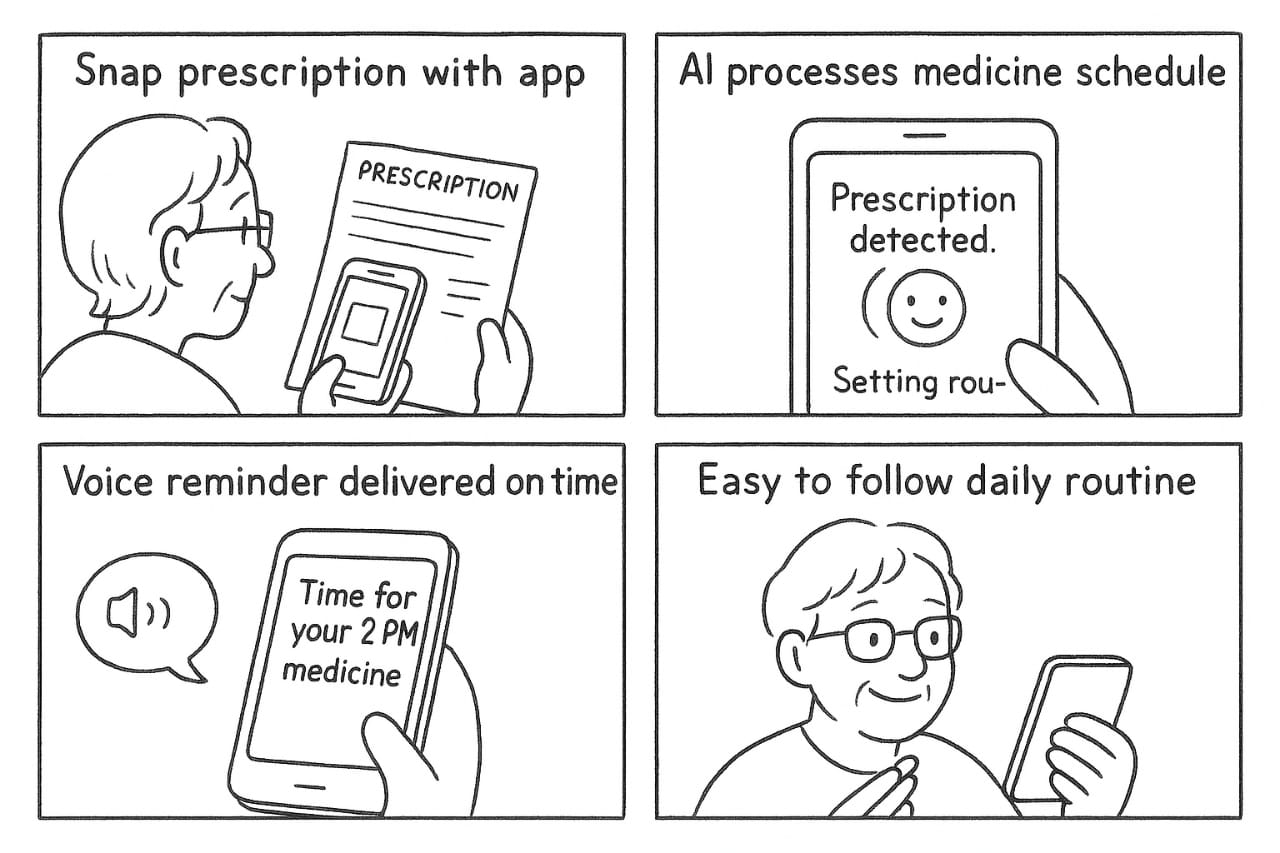
\includegraphics[width=0.3\linewidth]{Figures/initial uses.jpg}
  \caption{Initial Usage}
  \label{fig:fig1}
\end{figure}

\begin{figure}[h!]
  \centering
  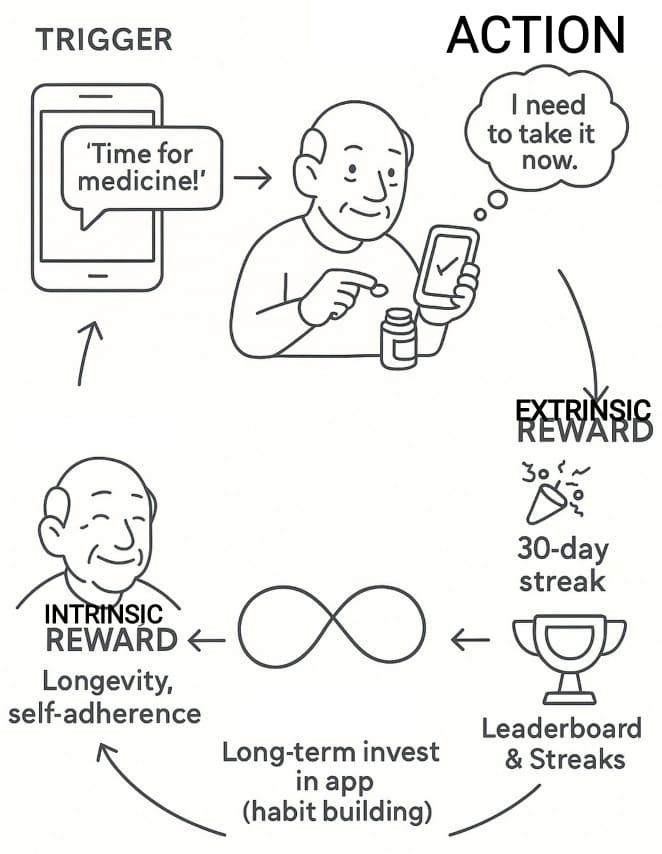
\includegraphics[height=6.5cm, width=0.3\linewidth]{Figures/main figure.jpg}
  \caption{Gamifying medication
adherence}
  \label{fig:fig2}
\end{figure}






\subsubsection{Designing for irregularity: }
Another line of work is explicitly designing for disruption. This might
include travel modes, event-based triggers, or adaptive rescheduling
features. Longitudinal field studies could evaluate whether such systems
hold up when life gets messy, rather than under ideal conditions.


\subsubsection{Caregiver–elder co-design: }
Further studies should bring both elders and caregivers into co-design
processes. \cite{10.1145/3613904.3642595} Questions worth pursuing: how should
control be shared? What permissions feel supportive versus intrusive?
How do cultural norms shape these dynamics? Understanding these issues
will help create systems that fit real caregiving relationships.

\subsubsection{Inclusive, low-tech prototypes: }
Future prototypes should push beyond the smartphone. \cite{10.1145/3594739.3610764}
Offline voice devices, SMS-to-voice bridges, or hybrid physical--digital
systems could all be tested. Research in this direction would expand the
reach of HCI to communities that rarely appear in health-tech studies
but face significant barriers.

\subsubsection{Building trust in App-based solutions: }
Lastly, work remains on trustworthiness. A lot of our participants were
unfamiliar with such solutions due to lack of accessibility and exposure
to technology. Even if we build the most cutting edge state of the art
solution, the question is not just whether the system works, but whether
people believe it works for them. \cite{10.3389/fdgth.2025.1523070}

\subsection{Limitations}
Several limitations must be acknowledged about our study. The study
sample was modest---26 participants from a specific cultural setting.
The findings therefore, should be read as situated, not universal.
Further research in different regions and caregiving arrangements is
needed. The data also relies on interviews rather than extended
observation. Interviews may capture attitudes and stories but they
cannot reveal all the small intricacies of adherence and forgetting or
missing. Observational or contextual inquiry-based studies would add
even further depth. Our exploration of AI systems was necessarily
speculative. Participants responded to scenarios rather than actual
built products or apps. While this elicited hopes and confusion,
real-world trials might reveal very different behaviors. Prototyping and
deployment studies are the next essential steps, based on the design
directions we mentioned before.

Gamification may be an exciting niche technique that is being adopted by
many other applications nowadays, but a lot of the participants in the
study evidently lack the exposure to technology, so we cannot certainly
say for sure they would really get hooked into the habit loop and adopt
such solutions as a healthy companion for their medication routines.

Finally, interpretation always involves subjectivity. Although analysis
was checked across researchers, our perspectives shaped the themes we
highlight. The contribution here is not universal law but a grounded
account of how these particular participants understand medication
adherence.

\section{Phase Two: Evaluation of the Implemented Prototype}

\subsection{From Formative Insight to Working System}
The formative study reported above was necessarily speculative: participants
reasoned about a reminder system that did not yet exist, responding to
scenarios and possibilities rather than to a product they had held in their
hands. Building on the design directions that emerged from that
work---particularly the call to support routine rather than override it, to
keep caregivers involved, and to make adherence feel like less of a
burden---we built and deployed a functioning voice- and visual-reminder
application with an accompanying streak/score-based tracking feature. This
section reports a second, evaluative phase of the study: semi-structured
interviews conducted after a period of real-world use of the app, intended to
test whether the concerns and hopes raised in Phase One held up once a real
system entered participants' daily lives.

\subsection{Methodology}

\subsubsection{Participants}
We interviewed six participants (four men, two women; ages 24--50, $M
\approx 29$) who had used the prototype for a period ranging from several
days to approximately three weeks prior to interview. Five participants were
young adults (24--26) who managed their own medication independently; one
participant, a 50-year-old woman managing diabetes, hypertension, and a
post-operative eye-medication regimen, was onboarded to the app with the
help of her adult daughter and represents a participant closer in profile to
the older-adult population centered in Phase One. Data collection for this
phase is ongoing; we report here on the first six interviews analyzed, with
additional interviews to be incorporated in a subsequent revision.

\subsubsection{Data Collection}
As in Phase One, we conducted semi-structured interviews, this time
organized around two parts: (1) participants' experience setting up and
living with the reminder and scheduling features, and (2) their experience
with the app's scoring/streak tracking feature specifically. Interviews were
conducted in a mix of Bangla and English, consistent with participants'
own code-switching in daily speech, and were audio recorded and transcribed.

\subsubsection{Data Analysis}
We followed the same reflexive thematic analysis approach used in Phase One.
Transcripts were read closely and open-coded, after which codes
were clustered into candidate themes and iteratively refined against the
data. Where relevant, we explicitly cross-referenced emerging Phase Two
codes against the Phase One themes (memory and dignity, everyday disruption,
family and care networks, and aspirations for technology) to assess where
the deployed system confirmed, complicated, or diverged from what
participants had earlier imagined.

\subsection{Findings}

\subsubsection{From External Aid to Internalized Habit}
A theme largely inaccessible in Phase One's hypothetical framing---because
it depends on sustained real-world use---was the gradual internalization of
timing that several participants described. What began as dependence on the
app's alarm evolved, for some, into an anticipatory sense of when medication
was due. One participant described this directly:

\emph{``After using it [the app], the biggest change was the discipline...
even before the reminder notification comes I do get a sign that now I am
forgetting something.''} (Subrata, 24)

A university student described a similar arc, in which the notification
scaffolded a habit that eventually became self-sustaining:

\emph{``I have trained my brain so that whenever a notification pops up...
I used to check my phone. But after it became a habit, I didn't have to
check my phone because my brain got trained from it.''} (Shuvo, 24)

Even participants who still described themselves as reliant on the alarm
characterized that reliance as a positive, low-effort routine rather than a
burden: \emph{``I'd say 90\%, because when the alarm rings, I take the
medicine... it's become a habit of mine that I remember around that
time.''} (Nijhum, 26)

This pattern complicates the Phase One finding that framed personal memory
as a matter of dignity and external aids as a potential threat to autonomy.
In use, participants did not describe the app as replacing their memory or
undermining their independence; rather, several described it as training or
restoring a kind of internal reliability they had previously lost to a busy
or irregular schedule. This suggests the earlier tension between
``relying on oneself'' and ``relying on a tool'' may be less binary in
practice than participants anticipated in the abstract---the tool can
become, over time, indistinguishable from the habit itself.

\subsubsection{Trust Built Through Self-Verification}
An unanticipated behavior that recurred across several participants was a
period of active, self-initiated verification before they trusted the
system. Participants described deliberately testing the app's alarms before
relying on them for actual doses:

\emph{``Before I fully believed in it, I did a 30-minute timer test, and it
worked. It was a good experience.''} (Subrata, 24)

\emph{``We first set it with a 15--20 minute window, then watched to see if
it actually worked after that time.''} (Ranjana Bhowmik, 50)

\emph{``The first day I used this app, I checked to make sure it was
working correctly, but after that I saw it reminded me on time, so I didn't
have any more problems.''} (Tanjim, 26)

This was not something Phase One's hypothetical framing could have
surfaced, since it depends on the existence of a real system to test against.
It suggests that trust in a reminder system is not established at the
moment of setup, but earned incrementally through a short probationary
period during which users independently audit the system's reliability. This
has a direct design implication: onboarding flows might productively surface
this verification instinct rather than working around it, for instance by
offering an explicit ``test my reminder'' function during setup.

\subsubsection{The App as a Safety Net Amid Everyday Disruption}
Phase One's finding that adherence is fragile under disruption---travel,
social events, and busy days---was one of the more consequential contributions
of the formative study. Phase Two provides a first empirical test of whether
a voice/visual reminder system meaningfully offsets that fragility, and the
evidence, drawn from participants' own disruption stories, is encouraging.

A participant described a trip that would, in the Phase One accounts, have
been a canonical case of missed medication:

\emph{``While I was traveling to Chittagong, I was out all day and had
completely forgotten about my medicine. But then I heard it ring, and I
realized it was time. I quickly took the medicine out of my bag and took
it.''} (Tanjim, 26)

Another participant described a near-miss during a mundane but disruptive
commute:

\emph{``One day, returning from college, the traffic was so bad that after
getting home I nearly forgot to take my daily medicine. At that time the
app notification came and I got reminded.''} (Subrata, 24)

A participant visiting family described a similar rescue from a socially
absorbing occasion---precisely the kind of scenario (a family gathering) that
produced one of Phase One's most serious adverse events, a caregiver's
account of her diabetic mother's health deteriorating after a missed dose
at a wedding:

\emph{``It was the day I went to my sister's home with my family. We had
so much fun that I didn't think about my routine at all, but the app always
reminded me when it was time, and I was so relieved.''} (Shuvo, 24)

For the one participant managing a genuinely complex, multi-drug,
multi-interval regimen following eye surgery, the app appeared to absorb
what had previously been a considerable mental load:

\emph{``My mental burden has reduced a lot, because I have to remember so
many medicines and follow their timing---that's a kind of hard thing to
manage. But since using this, I don't face that problem with taking
medicine anymore.''} (Ranjana Bhowmik, 50)

Taken together, these accounts suggest that the specific failure modes
identified in Phase One---travel, social occasions, competing demands on
attention---are precisely the situations in which participants found the
app most valuable, rather than situations in which it, too, failed. This is
a meaningful validation of the formative work, though we treat it
cautiously given the small and skewed sample (Section~\ref{sec:phase2-limitations}).

\subsubsection{Gamification as a Double-Edged Motivator}
Phase One participants had not interacted with any scoring or streak
mechanic, so their aspirations for such a feature were speculative. In
practice, the scoring/streak system produced consistently positive affect,
but with a more complicated relationship to pressure and loss than a purely
positive read would suggest.

Most participants described the score as a source of encouragement rather
than obligation:

\emph{``It felt good. It encouraged me---if I maintain this, my score will
get higher, more like a game.''} (Nijhum, 26)

\emph{``I would see my points increasing every day after taking my
medicine... my point increasing became a kind of encouragement to
me.''} (Ranjana Bhowmik, 50)

One participant connected daily score gains to a strong positive
association with reward, describing feeling as though he was working
toward buying a car after seeing his points grow (Tanjim, 26)---an
exaggeration, but a telling one about the emotional charge the mechanic
carried for at least some users.

However, several participants also described a real, if manageable, sting
when a streak was broken. This was most vivid in one account:

\emph{``At first I really felt that I had lost an important part of my
life, since I'd been doing this for 20--25 days and now it was broken. But
then I thought, I can do it again---this time with more patience and
discipline.''} (Subrata, 24)

Ranjana Bhowmik described a similar dynamic in terms of pressure to avoid
resetting to zero: \emph{``If it goes down to zero completely, that feels a
little frustrating... so there was always a bit of pressure, a bit of
self-motivation needed, so that I could maintain it.''} Nijhum expressed a
comparable, more muted version of the same tension: a resulting streak-reset
would be \emph{``a little frustrating,''} even though he did not describe it
as stressful in a sustained way.

Notably, not every participant experienced the score as consequential to
their underlying behavior. Tanjim, whose account emphasized that medication
was non-negotiable regardless of any app feature (\emph{``I have to take my
medicine to survive''}), treated the score as a pleasant bonus layered on
top of an already-settled commitment rather than a driver of it. Two
participants (Sumaiya Islam and Tanjim) also independently described the
score as tied to a redeemable, monetized incentive---explicitly describing
points as convertible into discounts or money---which appeared to add a
tangible, transactional layer to the gamification that is distinct from the
purely symbolic score/streak mechanic other participants described. This
detail should be confirmed against the actual feature specification, but if
accurate, it suggests the system's incentive design combines symbolic
gamification (streaks, points-as-progress) with a more concrete
extrinsic reward (points-as-currency), and future analysis should treat
these as analytically distinct mechanisms rather than a single
``gamification'' effect.

Together, these accounts suggest gamification functioned largely as
intended---as encouragement rather than coercion---but was not
motivationally neutral. The mild grief or frustration associated with a
broken streak, while not reported as harmful, is worth monitoring
longitudinally, particularly for users managing chronic, high-stakes
conditions where guilt or anxiety around ``failure'' could plausibly
undermine rather than support long-term adherence.

\subsubsection{Family Still Present, Roles Renegotiated}
Phase One identified family members as central, active participants in
medication management---as reminders, interpreters of prescriptions, and
emotional anchors. A natural question for Phase Two was whether a working
reminder app would displace this role. The evidence suggests it does not so
much displace it as relocate it.

For the one older participant in this sample, her daughter's involvement
shifted from an ongoing reminder role to a one-time onboarding role:

\emph{``I had some trouble setting it up myself, so my eldest daughter set
it up for me since she knows how to do these things.''} (Ranjana Bhowmik,
50)

Once configured, however, Ranjana Bhowmik described managing the day-to-day
tracking herself without difficulty, and her daughter's involvement
persisted in a new, socially reinforcing form: \emph{``My daughter would
also say, `look how much your score has gone up.'''} This small detail
echoes Phase One's finding that checking on medication was also a way
family members expressed care, and suggests that even a functioning,
largely self-sufficient system leaves room---and perhaps even creates new
occasions---for that expression to continue.

Ranjana Bhowmik also explicitly requested a feature that would formalize
this social dimension:

\emph{``If I could add my relatives here and see their scores too, that
would be more exciting for me... since we're middle-aged, remembering to
take medicine is a bit of a problem, so seeing this would encourage us,
and we wouldn't feel so much pressure.''}

This is a direct, participant-originated design request that extends
Phase One's caregiver-inclusion principle into a concrete feature: shared or
comparative tracking across a family unit, rather than tracking that is
strictly individual and private.

A related but distinct pattern appeared among the younger participants, for
whom the app appeared to substitute for a family reminder role that had
previously been necessary. Sumaiya Islam described this shift explicitly:
\emph{``Family members, close friends would remind me... but since the app
came along, it's become a kind of self-reminder.''} Tanjim described
something similar, noting that he no longer needed his mother or a written
note on the medicine box to remember his doses. For these participants, the
app did not add a new caregiver-facing feature so much as reduce their
reliance on informal reminders from people around them---suggesting that the
app's role relative to family support may differ meaningfully by
participant age, living situation, and complexity of regimen, a distinction
Phase One's largely older-adult sample could not fully anticipate.

\subsubsection{Residual Friction Points}
Consistent with Phase One's finding that usability flaws can undermine
otherwise promising technology, participants raised several concrete, minor
friction points. Initial setup, while generally described as easy, took
longer than some participants expected or wanted: \emph{``It felt a bit
time-consuming. If it could be made a little faster, I think it would be
better.''} (Nijhum, 26) One participant found entering medicines
individually tedious: \emph{``I have to add medicines one by one. That's a
part that sometimes feels frustrating.''} (Subrata, 24) Another found the
volume of progress data mildly overwhelming, though not seriously
problematic: \emph{``the progress shows a lot of data, but that's not a big
problem.''} (Shuvo, 24) Finally, one participant suggested that the alarm
sound itself could be a source of irritation, particularly for someone
sleeping or occupied with an important task, and proposed replacing it with
music: \emph{``if instead of the alarm there were some interesting music,
that might be better... it wouldn't feel so disturbing.''} (Nijhum, 26)
None of these issues were described as significant enough to threaten
continued use, but they represent low-cost opportunities for refinement.

\subsection{Connecting Phase Two to Phase One}
Read alongside one another, the two phases of this study tell a coherent
story about the movement from imagined solution to lived experience.
Phase One's central claim---that memory is entangled with dignity and that
adherence is fragile under everyday disruption---is substantially supported
by Phase Two: participants describe the very disruptions Phase One warned
about (travel, social events, competing demands) as the moments where the
app proved most valuable, and describe the app's support in terms closer to
restored confidence than imposed dependence. At the same time, Phase Two
surfaces dynamics that a purely formative study could not have
anticipated: a self-directed trust-verification period before adoption,
the emotional weight of a broken streak, and a family role that persists
but relocates from ongoing reminding to onboarding and social witnessing.
Where Phase One raised gamification only as a design possibility, Phase Two
shows it working largely as intended, while also surfacing a real, if mild,
psychological cost to streak loss that designers should not dismiss simply
because participants describe it as manageable.

\subsection{Limitations of the Evaluation Phase}
\label{sec:phase2-limitations}
This phase carries limitations distinct from, and in some ways sharper
than, those of Phase One. Most importantly, the current sample
(\emph{n}~=~6) is small, skewed toward younger participants (five of six
aged 24--26), and includes only one participant who closely resembles the
older-adult population that motivated the original study. Phase One's
core population---older adults with lower digital literacy---is therefore
underrepresented in this evaluation so far, and the strongly positive
habituation and trust-building patterns reported here may not generalize
to users with less prior smartphone experience. Additional interviews with
older participants and caregivers are needed before these findings can be
read as a genuine test of the Phase One design directions, and are planned
as an extension of this analysis. The evaluation period was also relatively
short (days to a few weeks), which is sufficient to observe initial habit
formation but not long-term retention, disengagement, or the durability of
the trust-verification behavior described above. Finally, as in Phase One,
interpretation involved subjectivity, and the monetized-points detail
raised by two participants should be verified against the system's actual
design before being treated as a confirmed feature rather than a
participant impression.

\section{Conclusion}
This study advances HCI in three main ways. First, it reframes memory
from a weakness to a valued resource, demanding technologies that
scaffold rather than replace. Second, it shows that sticking to
medication is fragile and often disrupted, so systems should be built to
adapt and recover rather than follow rigid rules. Third, it points to
the value of voice-based, caregiver-inclusive tools that make access
easier for people who are excluded from app-based health technologies.

Our second, evaluative phase lends early empirical support to these
claims. Participants who used a working prototype described the
disruptive scenarios identified in Phase One---travel, social events,
irregular routines---as exactly the moments in which the system proved
most valuable, and described its support in terms of restored confidence
rather than diminished autonomy. At the same time, real use surfaced
dynamics a formative study alone could not: an initial period of active
trust-verification, a family role that persists but relocates from
reminding to onboarding and social encouragement, and a gamification
mechanic that motivates effectively but carries a real, if modest,
emotional cost when a streak breaks. These findings should be read as
early and provisional, drawn from a small and age-skewed sample, but they
mark a meaningful step from imagined design directions toward evidence
about how such a system behaves in people's actual lives.

In doing so, the study moves beyond the narrow problem of ``reminding.''
It reveals adherence as bound up with dignity, identity, family, and
circumstance. Designing for this space means working with, not against,
these complexities. Medication support is not just about taking pills on
time. It is about preserving autonomy, managing disruption, and honoring
the networks of care that sustain older adults. HCI has the opportunity
to build systems that do more than count doses. It can build
technologies that respect lives.
% The ``\verb|acmart|'' document class requires the use of the
% ``Libertine'' typeface family. Your \TeX\ installation should include
% this set of packages. Please do not substitute other typefaces. The
% ``\verb|lmodern|'' and ``\verb|ltimes|'' packages should not be used,
% as they will override the built-in typeface families.

% \section{Title Information}

% The title of your work should use capital letters appropriately -
% \url{https://capitalizemytitle.com/} has useful rules for
% capitalization. Use the {\verb|title|} command to define the title of
% your work. If your work has a subtitle, define it with the
% {\verb|subtitle|} command.  Do not insert line breaks in your title.

% If your title is lengthy, you must define a short version to be used
% in the page headers, to prevent overlapping text. The \verb|title|
% command has a ``short title'' parameter:
% \begin{verbatim}
%   \title[short title]{full title}
% \end{verbatim}

% \section{Authors and Affiliations}

% Each author must be defined separately for accurate metadata
% identification.  As an exception, multiple authors may share one
% affiliation. Authors' names should not be abbreviated; use full first
% names wherever possible. Include authors' e-mail addresses whenever
% possible.

% Grouping authors' names or e-mail addresses, or providing an ``e-mail
% alias,'' as shown below, is not acceptable:
% \begin{verbatim}
%   \author{Brooke Aster, David Mehldau}
%   \email{dave,judy,steve@university.edu}
%   \email{firstname.lastname@phillips.org}
% \end{verbatim}

% The \verb|authornote| and \verb|authornotemark| commands allow a note
% to apply to multiple authors --- for example, if the first two authors
% of an article contributed equally to the work.

% If your author list is lengthy, you must define a shortened version of
% the list of authors to be used in the page headers, to prevent
% overlapping text. The following command should be placed just after
% the last \verb|\author{}| definition:
% \begin{verbatim}
%   \renewcommand{\shortauthors}{McCartney, et al.}
% \end{verbatim}
% Omitting this command will force the use of a concatenated list of all
% of the authors' names, which may result in overlapping text in the
% page headers.

% The article template's documentation, available at
% \url{https://www.acm.org/publications/proceedings-template}, has a
% complete explanation of these commands and tips for their effective
% use.

% Note that authors' addresses are mandatory for journal articles.

% \section{Rights Information}

% Authors of any work published by ACM will need to complete a rights
% form. Depending on the kind of work, and the rights management choice
% made by the author, this may be copyright transfer, permission,
% license, or an OA (open access) agreement.

% Regardless of the rights management choice, the author will receive a
% copy of the completed rights form once it has been submitted. This
% form contains \LaTeX\ commands that must be copied into the source
% document. When the document source is compiled, these commands and
% their parameters add formatted text to several areas of the final
% document:
% \begin{itemize}
% \item the ``ACM Reference Format'' text on the first page.
% \item the ``rights management'' text on the first page.
% \item the conference information in the page header(s).
% \end{itemize}

% Rights information is unique to the work; if you are preparing several
% works for an event, make sure to use the correct set of commands with
% each of the works.

% The ACM Reference Format text is required for all articles over one
% page in length, and is optional for one-page articles (abstracts).

% \section{CCS Concepts and User-Defined Keywords}

% Two elements of the ``acmart'' document class provide powerful
% taxonomic tools for you to help readers find your work in an online
% search.

% The ACM Computing Classification System ---
% \url{https://www.acm.org/publications/class-2012} --- is a set of
% classifiers and concepts that describe the computing
% discipline. Authors can select entries from this classification
% system, via \url{https://dl.acm.org/ccs/ccs.cfm}, and generate the
% commands to be included in the \LaTeX\ source.

% User-defined keywords are a comma-separated list of words and phrases
% of the authors' choosing, providing a more flexible way of describing
% the research being presented.

% CCS concepts and user-defined keywords are required for for all
% articles over two pages in length, and are optional for one- and
% two-page articles (or abstracts).

% \section{Sectioning Commands}

% Your work should use standard \LaTeX\ sectioning commands:
% \verb|\section|, \verb|\subsection|, \verb|\subsubsection|,
% \verb|\paragraph|, and \verb|\subparagraph|. The sectioning levels up to
% \verb|\subsusection| should be numbered; do not remove the numbering
% from the commands.

% Simulating a sectioning command by setting the first word or words of
% a paragraph in boldface or italicized text is {\bfseries not allowed.}

% Below are examples of sectioning commands.

% \subsection{Subsection}
% \label{sec:subsection}

% This is a subsection.

% \subsubsection{Subsubsection}
% \label{sec:subsubsection}

% This is a subsubsection.

% \paragraph{Paragraph}

% This is a paragraph.

% \subparagraph{Subparagraph}

% This is a subparagraph.

% \section{Tables}

% The ``\verb|acmart|'' document class includes the ``\verb|booktabs|''
% package --- \url{https://ctan.org/pkg/booktabs} --- for preparing
% high-quality tables.

% Table captions are placed {\itshape above} the table.

% Because tables cannot be split across pages, the best placement for
% them is typically the top of the page nearest their initial cite.  To
% ensure this proper ``floating'' placement of tables, use the
% environment \textbf{table} to enclose the table's contents and the
% table caption.  The contents of the table itself must go in the
% \textbf{tabular} environment, to be aligned properly in rows and
% columns, with the desired horizontal and vertical rules.  Again,
% detailed instructions on \textbf{tabular} material are found in the
% \textit{\LaTeX\ User's Guide}.

% Immediately following this sentence is the point at which
% Table~\ref{tab:freq} is included in the input file; compare the
% placement of the table here with the table in the printed output of
% this document.

% \begin{table}
%   \caption{Frequency of Special Characters}
%   \label{tab:freq}
%   \begin{tabular}{ccl}
%     \toprule
%     Non-English or Math&Frequency&Comments\\
%     \midrule
%     \O & 1 in 1,000& For Swedish names\\
%     $\pi$ & 1 in 5& Common in math\\
%     \$ & 4 in 5 & Used in business\\
%     $\Psi^2_1$ & 1 in 40,000& Unexplained usage\\
%   \bottomrule
% \end{tabular}
% \end{table}

% To set a wider table, which takes up the whole width of the page's
% live area, use the environment \textbf{table*} to enclose the table's
% contents and the table caption.  As with a single-column table, this
% wide table will ``float'' to a location deemed more
% desirable. Immediately following this sentence is the point at which
% Table~\ref{tab:commands} is included in the input file; again, it is
% instructive to compare the placement of the table here with the table
% in the printed output of this document.

% \begin{table*}
%   \caption{Some Typical Commands}
%   \label{tab:commands}
%   \begin{tabular}{ccl}
%     \toprule
%     Command &A Number & Comments\\
%     \midrule
%     \texttt{{\char'134}author} & 100& Author \\
%     \texttt{{\char'134}table}& 300 & For tables\\
%     \texttt{{\char'134}table*}& 400& For wider tables\\
%     \bottomrule
%   \end{tabular}
% \end{table*}

% Always use midrule to separate table header rows from data rows, and
% use it only for this purpose. This enables assistive technologies to
% recognise table headers and support their users in navigating tables
% more easily.

% \section{Math Equations}
% You may want to display math equations in three distinct styles:
% inline, numbered or non-numbered display.  Each of the three are
% discussed in the next sections.

% \subsection{Inline (In-text) Equations}
% A formula that appears in the running text is called an inline or
% in-text formula.  It is produced by the \textbf{math} environment,
% which can be invoked with the usual
% \texttt{{\char'134}begin\,\ldots{\char'134}end} construction or with
% the short form \texttt{\$\,\ldots\$}. You can use any of the symbols
% and structures, from $\alpha$ to $\omega$, available in
% \LaTeX~\cite{Lamport:LaTeX}; this section will simply show a few
% examples of in-text equations in context. Notice how this equation:
% \begin{math}
%   \lim_{n\rightarrow \infty}x=0
% \end{math},
% set here in in-line math style, looks slightly different when
% set in display style.  (See next section).

% \subsection{Display Equations}
% A numbered display equation---one set off by vertical space from the
% text and centered horizontally---is produced by the \textbf{equation}
% environment. An unnumbered display equation is produced by the
% \textbf{displaymath} environment.

% Again, in either environment, you can use any of the symbols and
% structures available in \LaTeX\@; this section will just give a couple
% of examples of display equations in context.  First, consider the
% equation, shown as an inline equation above:
% \begin{equation}
%   \lim_{n\rightarrow \infty}x=0
% \end{equation}
% Notice how it is formatted somewhat differently in
% the \textbf{displaymath}
% environment.  Now, we'll enter an unnumbered equation:
% \begin{displaymath}
%   \sum_{i=0}^{\infty} x + 1
% \end{displaymath}
% and follow it with another numbered equation:
% \begin{equation}
%   \sum_{i=0}^{\infty}x_i=\int_{0}^{\pi+2} f
% \end{equation}
% just to demonstrate \LaTeX's able handling of numbering.

% \section{Figures}

% The ``\verb|figure|'' environment should be used for figures. One or
% more images can be placed within a figure. If your figure contains
% third-party material, you must clearly identify it as such, as shown
% in the example below.
% \begin{figure}[h]
%   \centering
%   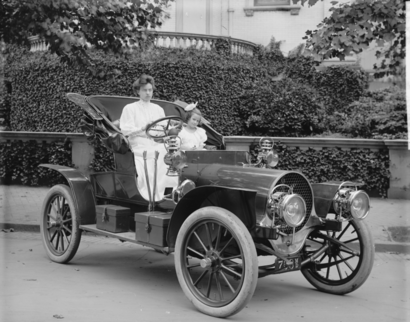
\includegraphics[width=\linewidth]{sample-franklin}
%   \caption{1907 Franklin Model D roadster. Photograph by Harris \&
%     Ewing, Inc. [Public domain], via Wikimedia
%     Commons. (\url{https://goo.gl/VLCRBB}).}
%   \Description{A woman and a girl in white dresses sit in an open car.}
% \end{figure}

% Your figures should contain a caption which describes the figure to
% the reader.

% Figure captions are placed {\itshape below} the figure.

% Every figure should also have a figure description unless it is purely
% decorative. These descriptions convey what’s in the image to someone
% who cannot see it. They are also used by search engine crawlers for
% indexing images, and when images cannot be loaded.

% A figure description must be unformatted plain text less than 2000
% characters long (including spaces).  {\bfseries Figure descriptions
%   should not repeat the figure caption – their purpose is to capture
%   important information that is not already provided in the caption or
%   the main text of the paper.} For figures that convey important and
% complex new information, a short text description may not be
% adequate. More complex alternative descriptions can be placed in an
% appendix and referenced in a short figure description. For example,
% provide a data table capturing the information in a bar chart, or a
% structured list representing a graph.  For additional information
% regarding how best to write figure descriptions and why doing this is
% so important, please see
% \url{https://www.acm.org/publications/taps/describing-figures/}.

% \subsection{The ``Teaser Figure''}

% A ``teaser figure'' is an image, or set of images in one figure, that
% are placed after all author and affiliation information, and before
% the body of the article, spanning the page. If you wish to have such a
% figure in your article, place the command immediately before the
% \verb|\maketitle| command:
% \begin{verbatim}
%   \begin{teaserfigure}
%     \includegraphics[width=\textwidth]{sampleteaser}
%     \caption{figure caption}
%     \Description{figure description}
%   \end{teaserfigure}
% \end{verbatim}

% \section{Citations and Bibliographies}

% The use of \BibTeX\ for the preparation and formatting of one's
% references is strongly recommended. Authors' names should be complete
% --- use full first names (``Donald E. Knuth'') not initials
% (``D. E. Knuth'') --- and the salient identifying features of a
% reference should be included: title, year, volume, number, pages,
% article DOI, etc.

% The bibliography is included in your source document with these two
% commands, placed just before the \verb|\end{document}| command:
% \begin{verbatim}
%   \bibliographystyle{ACM-Reference-Format}
%   \bibliography{bibfile}
% \end{verbatim}
% where ``\verb|bibfile|'' is the name, without the ``\verb|.bib|''
% suffix, of the \BibTeX\ file.

% Citations and references are numbered by default. A small number of
% ACM publications have citations and references formatted in the
% ``author year'' style; for these exceptions, please include this
% command in the {\bfseries preamble} (before the command
% ``\verb|\begin{document}|'') of your \LaTeX\ source:
% \begin{verbatim}
%   \citestyle{acmauthoryear}
% \end{verbatim}


%   Some examples.  A paginated journal article \cite{Abril07}, an
%   enumerated journal article \cite{Cohen07}, a reference to an entire
%   issue \cite{JCohen96}, a monograph (whole book) \cite{Kosiur01}, a
%   monograph/whole book in a series (see 2a in spec. document)
%   \cite{Harel79}, a divisible-book such as an anthology or compilation
%   \cite{Editor00} followed by the same example, however we only output
%   the series if the volume number is given \cite{Editor00a} (so
%   Editor00a's series should NOT be present since it has no vol. no.),
%   a chapter in a divisible book \cite{Spector90}, a chapter in a
%   divisible book in a series \cite{Douglass98}, a multi-volume work as
%   book \cite{Knuth97}, a couple of articles in a proceedings (of a
%   conference, symposium, workshop for example) (paginated proceedings
%   article) \cite{Andler79, Hagerup1993}, a proceedings article with
%   all possible elements \cite{Smith10}, an example of an enumerated
%   proceedings article \cite{VanGundy07}, an informally published work
%   \cite{Harel78}, a couple of preprints \cite{Bornmann2019,
%     AnzarootPBM14}, a doctoral dissertation \cite{Clarkson85}, a
%   master's thesis: \cite{anisi03}, an online document / world wide web
%   resource \cite{Thornburg01, Ablamowicz07, Poker06}, a video game
%   (Case 1) \cite{Obama08} and (Case 2) \cite{Novak03} and \cite{Lee05}
%   and (Case 3) a patent \cite{JoeScientist001}, work accepted for
%   publication \cite{rous08}, 'YYYYb'-test for prolific author
%   \cite{SaeediMEJ10} and \cite{SaeediJETC10}. Other cites might
%   contain 'duplicate' DOI and URLs (some SIAM articles)
%   \cite{Kirschmer:2010:AEI:1958016.1958018}. Boris / Barbara Beeton:
%   multi-volume works as books \cite{MR781536} and \cite{MR781537}. A
%   presentation~\cite{Reiser2014}. An article under
%   review~\cite{Baggett2025}. A
%   couple of citations with DOIs:
%   \cite{2004:ITE:1009386.1010128,Kirschmer:2010:AEI:1958016.1958018}. Online
%   citations: \cite{TUGInstmem, Thornburg01, CTANacmart}.
%   Artifacts: \cite{R} and \cite{UMassCitations}.

% \section{Acknowledgments}

% Identification of funding sources and other support, and thanks to
% individuals and groups that assisted in the research and the
% preparation of the work should be included in an acknowledgment
% section, which is placed just before the reference section in your
% document.

% This section has a special environment:
% \begin{verbatim}
%   \begin{acks}
%   ...
%   \end{acks}
% \end{verbatim}
% so that the information contained therein can be more easily collected
% during the article metadata extraction phase, and to ensure
% consistency in the spelling of the section heading.

% Authors should not prepare this section as a numbered or unnumbered {\verb|\section|}; please use the ``{\verb|acks|}'' environment.

% \section{Appendices}

% If your work needs an appendix, add it before the
% ``\verb|\end{document}|'' command at the conclusion of your source
% document.

% Start the appendix with the ``\verb|appendix|'' command:
% \begin{verbatim}
%   \appendix
% \end{verbatim}
% and note that in the appendix, sections are lettered, not
% numbered. This document has two appendices, demonstrating the section
% and subsection identification method.

% \section{Multi-language papers}

% Papers may be written in languages other than English or include
% titles, subtitles, keywords and abstracts in different languages (as a
% rule, a paper in a language other than English should include an
% English title and an English abstract).  Use \verb|language=...| for
% every language used in the paper.  The last language indicated is the
% main language of the paper.  For example, a French paper with
% additional titles and abstracts in English and German may start with
% the following command
% \begin{verbatim}
% \documentclass[sigconf, language=english, language=german,
%                language=french]{acmart}
% \end{verbatim}

% The title, subtitle, keywords and abstract will be typeset in the main
% language of the paper.  The commands \verb|\translatedXXX|, \verb|XXX|
% begin title, subtitle and keywords, can be used to set these elements
% in the other languages.  The environment \verb|translatedabstract| is
% used to set the translation of the abstract.  These commands and
% environment have a mandatory first argument: the language of the
% second argument.  See \verb|sample-sigconf-i13n.tex| file for examples
% of their usage.

% \section{SIGCHI Extended Abstracts}

% The ``\verb|sigchi-a|'' template style (available only in \LaTeX\ and
% not in Word) produces a landscape-orientation formatted article, with
% a wide left margin. Three environments are available for use with the
% ``\verb|sigchi-a|'' template style, and produce formatted output in
% the margin:
% \begin{description}
% \item[\texttt{sidebar}:]  Place formatted text in the margin.
% \item[\texttt{marginfigure}:] Place a figure in the margin.
% \item[\texttt{margintable}:] Place a table in the margin.
% \end{description}

% %%
% %% The acknowledgments section is defined using the "acks" environment
% %% (and NOT an unnumbered section). This ensures the proper
% %% identification of the section in the article metadata, and the
% %% consistent spelling of the heading.
% \begin{acks}
% To Robert, for the bagels and explaining CMYK and color spaces.
% \end{acks}

% %%
% %% The next two lines define the bibliography style to be used, and
% %% the bibliography file.
% \bibliographystyle{ACM-Reference-Format}
% \bibliography{sample-base}


% %%
% %% If your work has an appendix, this is the place to put it.
% \appendix

% \section{Research Methods}

% \subsection{Part One}

% Lorem ipsum dolor sit amet, consectetur adipiscing elit. Morbi
% malesuada, quam in pulvinar varius, metus nunc fermentum urna, id
% sollicitudin purus odio sit amet enim. Aliquam ullamcorper eu ipsum
% vel mollis. Curabitur quis dictum nisl. Phasellus vel semper risus, et
% lacinia dolor. Integer ultricies commodo sem nec semper.

% \subsection{Part Two}

% Etiam commodo feugiat nisl pulvinar pellentesque. Etiam auctor sodales
% ligula, non varius nibh pulvinar semper. Suspendisse nec lectus non
% ipsum convallis congue hendrerit vitae sapien. Donec at laoreet
% eros. Vivamus non purus placerat, scelerisque diam eu, cursus
% ante. Etiam aliquam tortor auctor efficitur mattis.

% \section{Online Resources}

% Nam id fermentum dui. Suspendisse sagittis tortor a nulla mollis, in
% pulvinar ex pretium. Sed interdum orci quis metus euismod, et sagittis
% enim maximus. Vestibulum gravida massa ut felis suscipit
% congue. Quisque mattis elit a risus ultrices commodo venenatis eget
% dui. Etiam sagittis eleifend elementum.

% Nam interdum magna at lectus dignissim, ac dignissim lorem
% rhoncus. Maecenas eu arcu ac neque placerat aliquam. Nunc pulvinar
% massa et mattis lacinia.

\bibliographystyle{ACM-Reference-Format}
\bibliography{sample-base}
\end{document}
\endinput
%%
%% End of file `sample-acmlarge.tex'.
